\documentclass{standalone}
\usepackage{tikz}
\usetikzlibrary{patterns, positioning}
\usepackage[sfdefault]{ClearSans} %% option 'sfdefault' activates Clear Sans as the default text font
\usepackage[T1]{fontenc}

\begin{document}
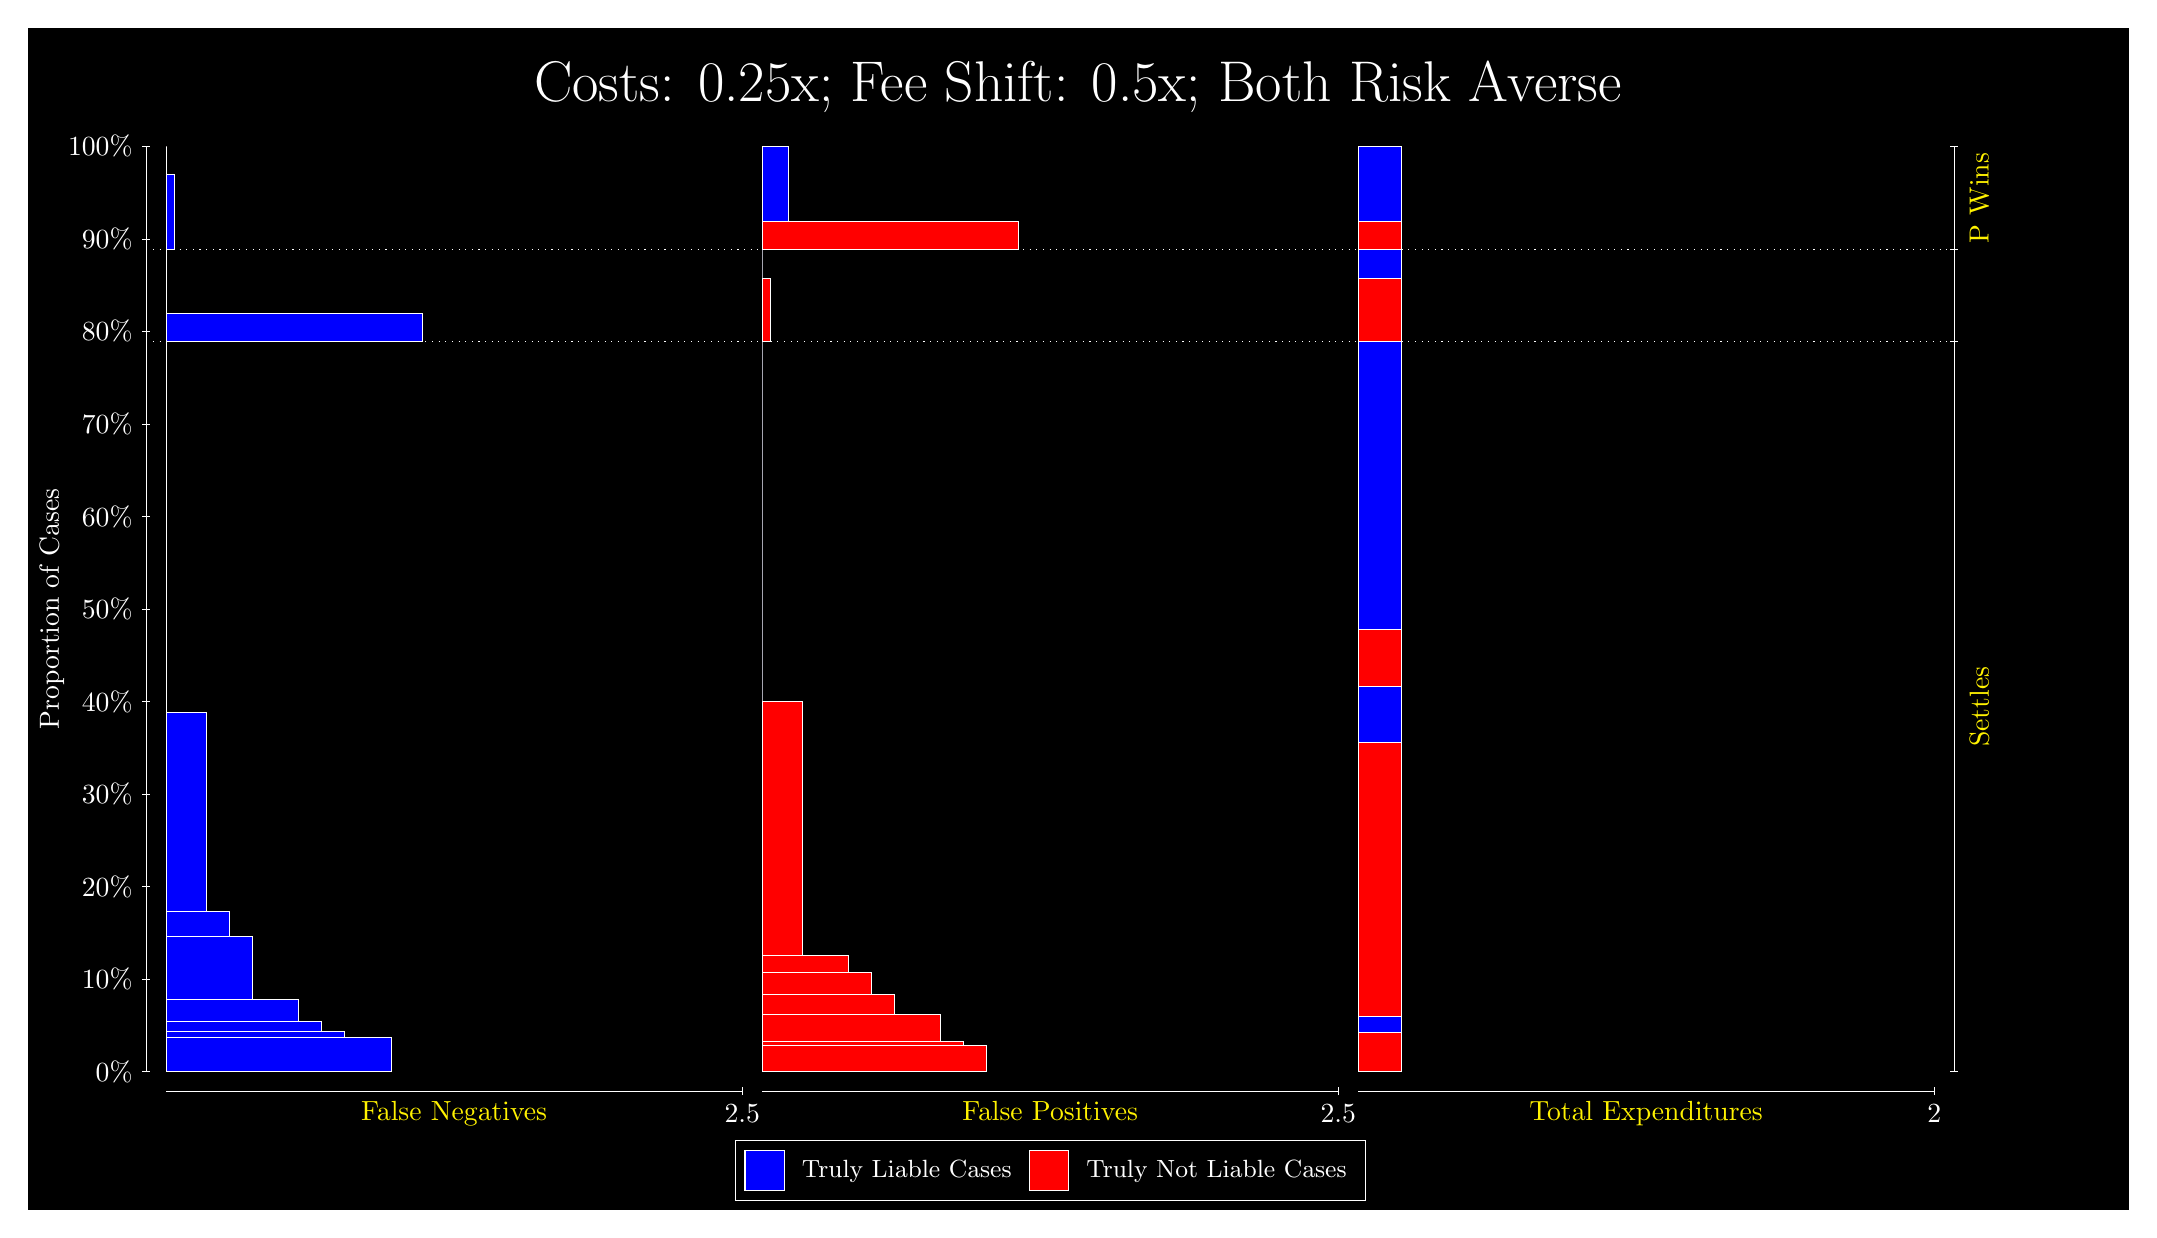
\begin{tikzpicture}
\draw[fill=black] (0,0) rectangle (26.667,15);
\draw[text=white] (0,13.5) rectangle (26.667,15) node[midway] {\huge Costs: 0.25x; Fee Shift: 0.5x; Both Risk Averse};
\draw[white, very thin] (1.5,1.75) -- (1.5,13.5);
\node[rotate=90, text=white, anchor=center] at (0.3, 7.625) {Proportion of Cases};
\draw[white, very thin] (1.45,1.75) -- (1.55,1.75);
\node[text=white, anchor=east] at (1.45, 1.75) {0\%};
\draw[white, very thin] (1.45,2.925) -- (1.55,2.925);
\node[text=white, anchor=east] at (1.45, 2.925) {10\%};
\draw[white, very thin] (1.45,4.1) -- (1.55,4.1);
\node[text=white, anchor=east] at (1.45, 4.1) {20\%};
\draw[white, very thin] (1.45,5.275) -- (1.55,5.275);
\node[text=white, anchor=east] at (1.45, 5.275) {30\%};
\draw[white, very thin] (1.45,6.45) -- (1.55,6.45);
\node[text=white, anchor=east] at (1.45, 6.45) {40\%};
\draw[white, very thin] (1.45,7.625) -- (1.55,7.625);
\node[text=white, anchor=east] at (1.45, 7.625) {50\%};
\draw[white, very thin] (1.45,8.8) -- (1.55,8.8);
\node[text=white, anchor=east] at (1.45, 8.8) {60\%};
\draw[white, very thin] (1.45,9.975) -- (1.55,9.975);
\node[text=white, anchor=east] at (1.45, 9.975) {70\%};
\draw[white, very thin] (1.45,11.15) -- (1.55,11.15);
\node[text=white, anchor=east] at (1.45, 11.15) {80\%};
\draw[white, very thin] (1.45,12.325) -- (1.55,12.325);
\node[text=white, anchor=east] at (1.45, 12.325) {90\%};
\draw[white, very thin] (1.45,13.5) -- (1.55,13.5);
\node[text=white, anchor=east] at (1.45, 13.5) {100\%};

\draw[white, very thin] (24.457,1.75) -- (24.457,13.5);
\draw[white, very thin] (24.407,1.75) -- (24.507,1.75);
\node[anchor=west] at (24.407, 1.75) {};
\draw[white, very thin] (24.407,11.018) -- (24.507,11.018);
\node[anchor=west] at (24.407, 11.018) {};
\draw[white, very thin] (24.407,12.187) -- (24.507,12.187);
\node[anchor=west] at (24.407, 12.187) {};
\draw[white, very thin] (24.407,13.5) -- (24.507,13.5);
\node[anchor=west] at (24.407, 13.5) {};

\draw[white, very thin, fill=blue] (1.75,1.75) rectangle (4.6044,2.184);
\draw[white, very thin, fill=blue] (1.75,2.184) rectangle (4.0188,2.2597);
\draw[white, very thin, fill=blue] (1.75,2.2597) rectangle (3.7261,2.3865);
\draw[white, very thin, fill=blue] (1.75,2.3865) rectangle (3.4333,2.662);
\draw[white, very thin, fill=blue] (1.75,2.662) rectangle (2.8478,3.4625);
\draw[white, very thin, fill=blue] (1.75,3.4625) rectangle (2.5551,3.7887);
\draw[white, very thin, fill=blue] (1.75,3.7887) rectangle (2.2623,6.3132);
\draw[white, very thin, fill=red] (1.75,6.3132) rectangle (1.75,11.018);
\draw[white, very thin, fill=blue] (1.75,11.018) rectangle (5.0069,11.377);
\draw[white, very thin, fill=red] (1.75,11.377) rectangle (1.75,12.187);
\draw[white, very thin, fill=blue] (1.75,12.187) rectangle (1.8598,13.14);
\draw[white, very thin, fill=red] (1.75,13.14) rectangle (1.75,13.5);
\draw[white, very thin, fill=red] (9.3189,1.75) rectangle (12.173,2.0851);
\draw[white, very thin, fill=red] (9.3189,2.0851) rectangle (11.88,2.1296);
\draw[white, very thin, fill=red] (9.3189,2.1296) rectangle (11.588,2.4727);
\draw[white, very thin, fill=red] (9.3189,2.4727) rectangle (11.002,2.7373);
\draw[white, very thin, fill=red] (9.3189,2.7373) rectangle (10.709,3.0152);
\draw[white, very thin, fill=red] (9.3189,3.0152) rectangle (10.417,3.2311);
\draw[white, very thin, fill=red] (9.3189,3.2311) rectangle (9.8312,6.4548);
\draw[white, very thin, fill=blue] (9.3189,6.4548) rectangle (9.3189,11.018);
\draw[white, very thin, fill=red] (9.3189,11.018) rectangle (9.4287,11.828);
\draw[white, very thin, fill=blue] (9.3189,11.828) rectangle (9.3189,12.187);
\draw[white, very thin, fill=red] (9.3189,12.187) rectangle (12.576,12.547);
\draw[white, very thin, fill=blue] (9.3189,12.547) rectangle (9.6482,13.5);
\draw[white, very thin, fill=red] (16.888,1.75) rectangle (17.437,2.2437);
\draw[white, very thin, fill=blue] (16.888,2.2437) rectangle (17.437,2.4463);
\draw[white, very thin, fill=red] (16.888,2.4463) rectangle (17.437,5.9347);
\draw[white, very thin, fill=blue] (16.888,5.9347) rectangle (17.437,6.6441);
\draw[white, very thin, fill=red] (16.888,6.6441) rectangle (17.437,7.3668);
\draw[white, very thin, fill=blue] (16.888,7.3668) rectangle (17.437,11.018);
\draw[white, very thin, fill=red] (16.888,11.018) rectangle (17.437,11.828);
\draw[white, very thin, fill=blue] (16.888,11.828) rectangle (17.437,12.187);
\draw[white, very thin, fill=red] (16.888,12.187) rectangle (17.437,12.547);
\draw[white, very thin, fill=blue] (16.888,12.547) rectangle (17.437,13.5);
\draw[white, dotted] (1.5,11.018) -- (24.457,11.018);
\draw[white, dotted] (1.5,12.187) -- (24.457,12.187);
\draw[white, very thin] (1.75,1.5) -- (9.0689,1.5);
\node[text=yellow, anchor=north] at (5.4094, 1.5) {False Negatives};
\draw[white, very thin] (9.0689,1.45) -- (9.0689,1.55);
\node[text=white, anchor=north] at (9.0689, 1.45) {2.5};

\draw[white, very thin] (9.3189,1.5) -- (16.638,1.5);
\node[text=yellow, anchor=north] at (12.978, 1.5) {False Positives};
\draw[white, very thin] (16.638,1.45) -- (16.638,1.55);
\node[text=white, anchor=north] at (16.638, 1.45) {2.5};

\draw[white, very thin] (16.888,1.5) -- (24.207,1.5);
\node[text=yellow, anchor=north] at (20.547, 1.5) {Total Expenditures};
\draw[white, very thin] (24.207,1.45) -- (24.207,1.55);
\node[text=white, anchor=north] at (24.207, 1.45) {2};

\node[text=yellow, centered, rotate=90] at (24.777, 6.384) {Settles};

\node[text=yellow, centered, rotate=90] at (24.777, 12.844) {P Wins};

\draw (12.978300999999998,1.5) node[draw=none] (baseCoordinate) {};
\begin{scope}[align=center]
        \matrix[scale=0.5, draw=white, below=0.5cm of baseCoordinate, nodes={draw}, column sep=0.1cm]{
            \node[rectangle, draw, minimum width=0.5cm, minimum height=0.5cm, fill=blue] {}; &
            \node[draw=none, font=\small, text=white] (B) {Truly Liable Cases}; &
            \node[rectangle, draw, minimum width=0.5cm, minimum height=0.5cm, fill=red] {}; &
            \node[draw=none, font=\small, text=white] (B) {Truly Not Liable Cases}; \\
            };
\end{scope}

\end{tikzpicture}
\end{document}